\section{Results}\label{sec:results}
\subsection{singles and pair questions}
We first test the single and pair questions, comparing two types of Llama-8B models: Llama-3.1 and AstroSage \citep{haan2025_astrosage}, a Llama-3.1 model that was fine-tuned specifically on arXiv astrophysics papers.~\Cref{tab:basemodel} shows the comparison on both datasets. Single and pair descriptions are scored by the verifier, which extracts every numeric and categorical claim from the generated text and checks it against the catalog: \emph{numeric accuracy} is the fraction of stated values within a per-quantity tolerance of the catalog value, and \emph{qualitative} (single) or \emph{relational} (pair) accuracy is the fraction of class words or comparisons that match it (tolerances and definitions in \Cref{app:eval}). While both models show high performance on both tasks, Astrosage retains a small gain over the vanilla model in seven of the eight cells, across both datasets, which implies that textual domain knowledge is helpful for those tasks. Therefore, the Astrosage model was chosen for further analysis. 
\subsection{scientific reasoning tasks} Single and pair questions consists of description and simple comparisons and requires almost no reasoning beyond the basic properties. It is also similar to the protein description tasks as in  \cite{Dotan2026_betadescribe}, and therefore it is not surprising that an LLM performs well on such questions. Next, we test the performance on questions that requires some form of scientific reasoning. As mentioned in~\Cref{sec:data}, those are finding the odd member of a group of stars, and judging whether a galaxy's shape agrees with its star-formation history. The rest of the paper focuses on those tasks.~\Cref{tab:headboth} shows the results of the two reasoning tasks. \Cref{fig:examples} shows one example generated description for each task. The two tasks behave differently. On stars, the narrator alone, reading only the data tokens, fails: it names the odd member and its property in only a third of the groups. On galaxies, the narrator alone succeeds: trained with LoRA, it gives the right verdict for $97$--$99\%$ of galaxies. Interestingly, full fine-tuning performs slightly worse than LoRA, especially on quiescent galaxies. 

Before adding anything to the stellar narrator, we check whether its failure is a failure of information. A cross-fit linear probe on the same aligned features, asked to rank the members of a group, matches what the true catalog values achieve (rank-1 $0.660$ from the shared subspace and $0.686$ from the full feature, against $0.660$ for the catalog itself; \Cref{sec:appendix}). The signal the task needs is present in the features the model reads, so the failure is in the readout and not in the representation. The last column of \Cref{tab:headboth} adds the head token (see~\Cref{sec:data}). In the stellar case the head is a flow matching model that was trained to learn the joint distribution of the aligned features and catalog labels, conditioned on the rest of the group. In the galaxy case, it is a cross-modal predictor trained to predict one modality from the other. On stars, the head narrator doubles the score ($0.33 \to 0.66$). On galaxies, it is no better than a narrator trained the same way without the token (\Cref{app:2x2}). The stellar narrator without a head was fully fine-tuned while the head narrator was trained with LoRA, and the matching stellar control (LoRA without a head) has not been run (\Cref{sec:limitations}). \todo{run the missing experiment}

The asymmetry in performance, together with the results in~\Cref{tab:basemodel}, points to the number of objects in the question as the important factor for successful generation of the \emph{narrator}. The galaxy verdict concerns a single object and follows from two of its own properties, its shape and whether it still forms stars, which the narrator can read from that galaxy's tokens. Even though morphology-SFH disagreement is deeper than mere description, the \emph{narrator} still performs almost perfectly. In the stellar case, finding the odd star requires comparing every member with the rest of the group, a computation over the whole set that no single star's tokens contain. The narrator's strong performance on single and pair questions supports the hypothesis that population-related questions are inherently more challenging for the narrator. To test this, we vary only the number of stars while keeping the question fixed:
the test groups contain between $4$ and $32$ stars, and \Cref{fig:groupsize} shows
the score as a function of group size. Here we count a description as correct if it
names \emph{any} star that truly has the odd property, together with that property:
the test groups designate one odd star, but larger groups more often contain a
second star with the same property ($24\%$ of groups with $4$ stars, $84\%$ with
$32$), and naming it is a true statement. Without the head, the score falls
steadily as the group grows, from $0.51$ with $4$ stars to $0.15$ with $32$
(Spearman $\rho=-0.21$, $p=10^{-13}$). With the head, it stays between $0.69$ and
$0.81$ at every size and does not decline. Counting only the designated star gives
the same picture at lower values (dotted lines). The difficulty of the stellar task
therefore grows with the number of objects the narrator must compare, and the head
narrator does not suffer from it. Because the two narrators also differ in training
(LoRA against full fine-tuning), part of this stability may come from the training
rather than the head (\Cref{sec:limitations}). Since every star adds the same number
of tokens, a larger group is also a longer input, and our data cannot separate the
two. Next, we perform two ablation tests for the stellar population task: whether the improvement from using the head comes from reasoning or memorization, and whether handing the \emph{narrator} the full catalog numbers prevents the failure.

\begin{figure}[t]
  \centering
  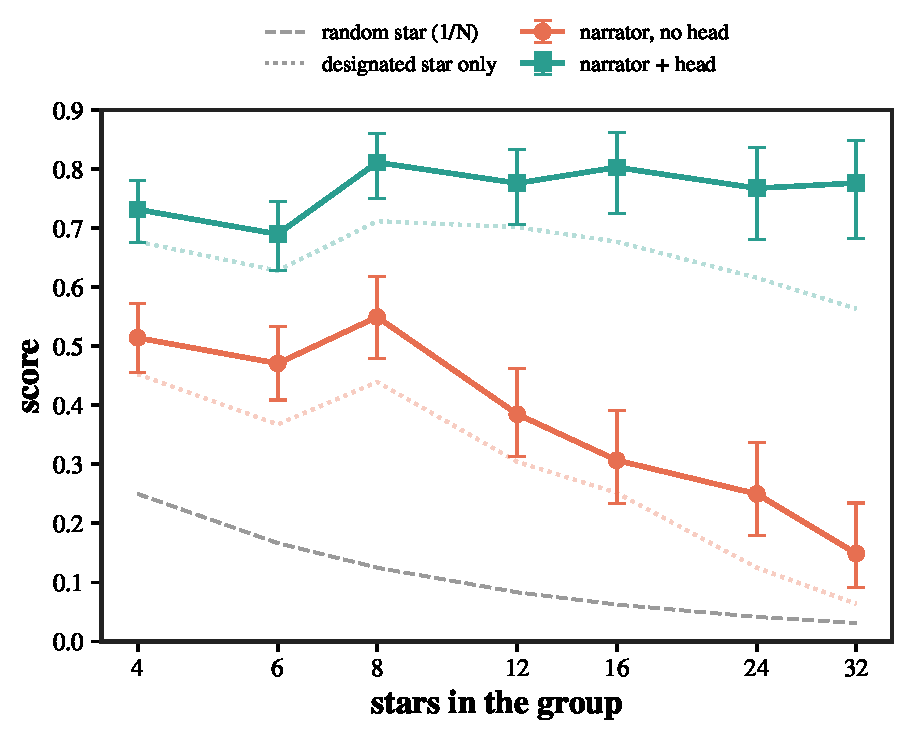
\includegraphics[width=0.8\linewidth]{figs/score_vs_group_size_lenient.pdf}
  \caption{\textbf{The stellar task becomes harder with the number of stars.}
  Fraction of groups in which the narrator names a star that truly has the odd
  property, and the property, as a function of the number of stars in the group,
  for the narrator without and with the head ($1{,}203$ test groups with an odd
  member). Error bars are $95\%$ intervals. Dotted lines: the same, counting only
  the designated odd star (the score of \Cref{tab:headboth}). Dashed line: the
  chance of picking the odd star at random ($1/N$); the score also requires the
  right property, so its chance level is lower still.}
  \label{fig:groupsize}
\end{figure}


\begin{figure*}[t]
  \centering
  % Example generations on the two reasoning tasks (verbatim narrator outputs, greedy).
% Galaxy: galaxy_id 601201, narrator trained with LoRA and no head token
%   (MultiLLM cache/galaxy_gen_eval/generations/lora_nohead_xmodal_eval.jsonl).
% Stars: test group population_451_N4 (MultiLLM cache/stellar_gen_eval_full/
%   generations/{astrosage8b,flow_astrosage8b_template}.jsonl).
\newcommand{\gOK}{{\color{teal!80!black}\,$\checkmark$}}
\newcommand{\gNO}{{\color{coral}\,$\times$}}
\newcommand{\hGood}[1]{{\setlength{\fboxsep}{0.6pt}\colorbox{paleteal}{\strut #1}}}
\newcommand{\hBad}[1]{{\setlength{\fboxsep}{0.6pt}\colorbox{palecoral}{\strut #1}}}
\tcbset{exbox/.style={colback=white, boxrule=0.6pt, arc=1.5pt,
  left=3pt, right=3pt, top=2pt, bottom=2pt, fontupper=\footnotesize,
  fonttitle=\footnotesize\bfseries, coltitle=deepteal,
  toptitle=0.6pt, bottomtitle=0.6pt}}
\begin{minipage}[t]{0.47\textwidth}\vspace{0pt}
  \begin{tcolorbox}[exbox, colframe=neutral, colbacktitle=palegrey,
      title={Galaxy: does its shape agree with its history?}]
    \raggedright
    \textbf{Catalog.} Late-type disk ($P{=}0.75$); quiescent
    ($\log \mathrm{sSFR} = -11.6$); declining star-formation history.
    A disk that has stopped forming stars: shape and history
    \emph{disagree}.
  \end{tcolorbox}\vspace{-2pt}
  \begin{tcolorbox}[exbox, colframe=teal!80!black, colbacktitle=paleteal,
      title={Narrator (no head token)\gOK}]
    \raggedright
    A \hGood{quiescent} \hGood{late-type disk} --- a
    \hGood{cross-modal outlier}, because disks rarely quench while retaining
    their morphology. Its star-formation history is \hGood{declining}.
  \end{tcolorbox}
  {\scriptsize\color{neutral} Shape, star formation and verdict all match the
  catalog.}
\end{minipage}\hfill
\begin{minipage}[t]{0.5\textwidth}\vspace{0pt}
  \begin{tcolorbox}[exbox, colframe=neutral, colbacktitle=palegrey,
      title={Stars: which one does not belong?}]
    \centering
    \begin{tabular}{@{}clccc@{}}
      star & class & $T_\mathrm{eff}$ [K] & $\log g$ & $R$ [$R_\odot$] \\
      \hline
      0 & dwarf    & 5778 & 4.39 & 1.05 \\
      \hBad{1} & \hBad{\textbf{giant}} & \hBad{4662} & \hBad{\textbf{2.45}} & \hBad{\textbf{11.14}} \\
      2 & subgiant & 5628 & 3.89 & 2.00 \\
      3 & dwarf    & 5394 & 4.55 & 0.81 \\
    \end{tabular}
  \end{tcolorbox}\vspace{-2pt}
  \begin{tcolorbox}[exbox, colframe=coral, colbacktitle=palecoral,
      title={Narrator, no head\gNO}]
    \raggedright
    These 4 stars form a homogeneous population of field stars.
    \hBad{No anomalies detected} along the field-star axis.
  \end{tcolorbox}\vspace{-2pt}
  \begin{tcolorbox}[exbox, colframe=teal!80!black, colbacktitle=paleteal,
      title={Narrator $+$ head\gOK}]
    \raggedright
    Sample N=4: single stars. \hGood{index 1: a giant} [logg = 2.44 dex,
    R = 11.14 Rsun, logL = 1.72 log(Lsun), giant].
  \end{tcolorbox}
\end{minipage}

  \caption{\textbf{Example generations on the two reasoning tasks}, verbatim and
  decoded greedily. \emph{Left}: a quenched disk, whose shape and star-formation
  history disagree. The narrator trained without the head token states the shape,
  the star-formation state and the verdict correctly, as it does for $97$--$99\%$
  of test galaxies. \emph{Right}: a test group of four stars containing one giant.
  The narrator without the head reports no odd member; the narrator with the head
  names the giant, with values that match the catalog.}
  \label{fig:examples}
\end{figure*}


\begin{table}[h]\centering\small
\caption{\textbf{Base model: Llama-3.1-8B vs.\ AstroSage-8B}, identical
corpus, recipe and seed; rule-scored, greedy; the better model in bold.
Metrics: \emph{numeric acc.} = fraction of numbers the text states that fall
within tolerance of the catalog value; \emph{qualitative acc.} (single) =
fraction of class words (dwarf/giant, disk/elliptical, \ldots) that match
the catalog; \emph{relational acc.} (pair) = fraction of comparisons
(``hotter than'', ``more massive'') that match.
}
\label{tab:basemodel}
\begin{tabular}{llcc}
\toprule
 & metric & Llama-3.1-8B & AstroSage-8B \\
\midrule
\multicolumn{4}{l}{\emph{galaxies --- one object}}\\
 & numeric acc.\     & 0.822 & \textbf{0.826} \\
 & qualitative acc.\ & 0.812 & \textbf{0.835} \\
\multicolumn{4}{l}{\emph{galaxies --- pair}}\\
 & numeric acc.\     & 0.647 & \textbf{0.672} \\
 & relational acc.\  & \textbf{0.795} & 0.771 \\
\midrule
\multicolumn{4}{l}{\emph{stars --- one object}}\\
 & numeric acc.\     & 0.909 & \textbf{0.911} \\
 & qualitative acc.\ & 0.575 & \textbf{0.628} \\
\multicolumn{4}{l}{\emph{stars --- pair}}\\
 & numeric acc.\     & 0.784 & \textbf{0.801} \\
 & relational acc.\  & 0.858 & \textbf{0.883} \\
\bottomrule
\end{tabular}
\end{table}


\begin{table}[h]\centering\small
\caption{\textbf{The reasoning tasks.} Each row is one task and scorer; the
columns are narrators that differ in how they were trained and whether they read
the head token. Stars: the fraction of the $1{,}203$ test groups with an odd member
in which the text names it \emph{and} its property, scored by the verifier and by
the judge, which agree on the size of the effect. Galaxies: the fraction of test
galaxies with the correct agreement verdict (\Cref{sec:galaxyscore}), on the
$9{,}609$ star-forming and $1{,}068$ quiescent galaxies. The stellar narrator
trained with LoRA and no head token was not run (\Cref{sec:limitations}).}
\label{tab:headboth}
\begin{tabular}{llccc}
\toprule
 & & \multicolumn{2}{c}{narrator, no head token} & narrator $+$ head \\
\cmidrule(lr){3-4}
task & scorer & full fine-tune & LoRA & LoRA \\
\midrule
\emph{stars} --- name the odd member  & verifier & 0.245 & --- & \textbf{0.633} \\
\hspace{1em}and its property          & judge    & 0.332 & --- & \textbf{0.662} \\
\midrule
\emph{galaxies} --- shape vs.\ history, & star-forming & 0.980 & \textbf{0.988} & 0.986 \\
\hspace{1em}correct verdict             & quiescent    & 0.884 & 0.974 & \textbf{0.978} \\
\bottomrule
\end{tabular}
\end{table}




% Section 4.3 (token or training?) set aside until the stellar LoRA-without-head
% control is run; restore by deleting the \iffalse / \fi pair.
\iffalse
\subsection{is it the token, or the training that came with it?}\label{sec:tokenortraining}
The narrators with and without the head are two separately trained models, and
they differ in more than the token: the head narrator is trained with LoRA on a
frozen base model, while the narrator without it is fully fine-tuned. The gain in
\Cref{tab:headboth} could therefore come from the token or from the training.
The test that does not depend on training is to take the trained head narrator
and break its token at generation time, leaving everything else unchanged.
\Cref{tab:ablate} does this two ways: scrambling the token across the group, so
that it has the right statistics but describes a different star, and replacing
it with zeros.

\begin{table}[h]\centering\small
\caption{\textbf{Breaking the token at test time}, stellar group task, full test
set ($n{=}1{,}203$ groups with an odd member, greedy, judge-scored).
\emph{score} is the fraction of descriptions that name the true odd member and
its property. The last three rows are one trained model, the head narrator, with
its token intact or damaged at generation time; the first row is a separately
trained model.}
\label{tab:ablate}
\begin{tabular}{lc}
\toprule
 & score  \\
\midrule
narrator, trained without a head token & 0.332 \\
\midrule
head narrator, token zeroed      & 0.561  \\
head narrator, token scrambled   & 0.606 \\
head narrator, token intact      & \textbf{0.662}  \\
\bottomrule
\end{tabular}
\end{table}

Breaking the token costs the same model $0.056$ (scrambled) to $0.101$ (zeroed),
both significant, so what the token contains is read and used. Even with a broken
token, however, the head narrator stays far above the narrator trained without
one ($0.561$ against $0.332$). A zeroed token carries no information about the
group, so this gap is a difference between the two trained models, not something
the token supplies at test time: it comes from how the head narrator was trained
(LoRA on a frozen base instead of full fine-tuning, and alongside a head token),
and a test-time ablation cannot tell these apart.

On galaxies we ran the missing control: a narrator trained with LoRA and
\emph{no} head token (\Cref{tab:headboth}, \Cref{app:2x2}). It matches the head
narrator on quiescent galaxies ($0.974$ against $0.978$, not significant) and is
slightly better on star-forming ones ($0.988$ against $0.986$). The full
fine-tune is the outlier: on quiescent galaxies it gives the wrong verdict for
$12\%$ of them, mostly because it misreads whether the galaxy still forms stars
($9\%$ of quiescent galaxies). On galaxies,
then, the gain over the fully fine-tuned narrator comes from the training, not from
the token. The galaxy narrator does read its token, since scrambling it costs a
little on star-forming galaxies ($0.986 \to 0.978$), but the token adds nothing
the data tokens do not already provide; this is expected, since the galaxy head is
computed from the same image and star-formation embeddings the narrator reads.

For stars, the same control would require training a stellar narrator with LoRA
and no head token, about $700$--$1{,}100$ GPU-hours, which we have not yet done.
Until then, the stellar evidence supports a narrower claim: the head token's
content is worth $0.06$--$0.10$ of the $0.33$ gain, and the remaining $0.23$
coincides with a change in training that we cannot yet separate from the token.
\fi

\subsection{is this reasoning, or memorization?}\label{sec:memorization}
As described in \Cref{sec:data}, $99.2\%$ of the stars we evaluate on appear in
\emph{some} training description. That is the same for every narrator, so the
paired comparisons above are fair, but it leaves an obvious objection: the head
narrator might be recalling which star was called unusual
during training rather than working it out.

We test this directly, on the stellar track. From the test fold we keep only
groups whose odd member was \emph{never} an odd member anywhere in training:
the star may have been described many times, but never as the one that stands
out. Only $2.3\%$ of candidate groups survive that filter, leaving $1{,}000$.
If the head narrator is recalling, it should lose most of its advantage here. Table~\ref{tab:adversarial} shows this experiment. The advantage does not shrink where memorisation is
impossible; it grows. The head is worth $+0.469$ on this set against
$+0.330$ on the full test set, and the two narrators move in opposite directions
on it: the narrator without the head falls ($0.332 \to 0.279$) while the head
narrator does not. That is the opposite of what a memorization
explanation predicts.

\begin{table}[h]\centering\small
\caption{$1{,}000$ stellar groups whose odd member
was never an odd member in training, greedy, judge-scored. \emph{score} is the fraction of descriptions that name the
true odd member and its property; \emph{named} counts naming the odd member
regardless of property, and \emph{property} naming the right property regardless
of member.}
\label{tab:adversarial}
\begin{tabular}{lccc}
\toprule
 & score & named & property  \\
\midrule
narrator & 0.279 & 0.329 & 0.343  \\
narrator $+$ head   & \textbf{0.748} & \textbf{0.782} & \textbf{0.761}  \\
$\Delta$  & $+0.469$ & $+0.453$ & $+0.418$ \\
\bottomrule
\end{tabular}
\end{table}


% One caveat on reading the table. This set is deliberately harder than the full
% fold and its item mix is different, so only the within-set gap is quotable:
% compare $0.748$ to $0.279$, not to the $0.662$ of \Cref{tab:headboth}. Groups
% with no odd member are excluded throughout, here and everywhere else in the
% paper.

\subsection{giving the model the numbers as text}\label{sec:text}
If the features carry the signal and the model cannot use it, an obvious
alternative is to skip the features and hand the model the catalog numbers
directly. We test this on the stellar task. Each group is shown as a table with
one row per star, listing its catalog values (temperature, surface gravity,
metallicity, radius, mass, and others) together with the two catalog flags the
head also receives: whether the star is a binary and whether it belongs to an
open cluster. With these flags the table holds everything the head is given, so
the comparison is fair for all five kinds of odd star. The model sees two worked
examples and is asked, in words, to name the star that does not belong and the
property it differs in. We test two models: the base AstroSage-8B, without our
training, and Qwen3.5-27B, a larger general-purpose model. Each is tested twice:
answering directly, and reasoning step by step before answering.
\Cref{tab:text} compares them with the two narrators on the same $1{,}203$
groups.

No model that reads the numbers comes close to the narrator with the head
($0.662$). AstroSage reading the table reaches the second-best score ($0.473$),
but by naming most of the group ($82\%$ of the stars): naming the odd star among
them is then no better than chance ($0.92\times$). Asked to reason first, it
names few stars and scores $0.288$, below the narrator without the head. The
larger model is more selective: it names the odd star at about the same rate as
the head relative to the number of stars it names. However, it often gets the
odd star's property wrong, and scores $0.341$ answering directly and $0.324$
after reasoning, no different from the narrator without the head ($p{=}0.7$ in
both cases). In most groups ($94\%$) the larger model was still reasoning when
it reached the length limit of $4{,}096$ tokens and was made to answer from what
it had, so its reasoning result holds for this budget only. The gap to the head
also holds for every group size (\Cref{app:textsize}). Reading the numbers
lets a model describe the stars, but not reliably pick out the one that does
not belong.

\begin{table}[h]\centering\small
\caption{\textbf{Giving the model the numbers as text}, on the $1{,}203$ test
groups with an odd star (all five kinds), greedy. The text-reading models see
every catalog value plus the binary and open-cluster flags.
\emph{score} and \emph{named} are as in \Cref{tab:adversarial};
\emph{stars named} is the fraction of the group the text names; \emph{lift}
divides \emph{named} by it ($1.0$ = no better than naming that many stars at
random). Every text-reading model scores below the narrator with the head
($p<10^{-19}$, exact McNemar on \emph{score}).}
\label{tab:text}
\begin{tabular}{lcccc}
\toprule
 & score & named & lift & stars named \\
\midrule
AstroSage-8B, reads the table                & 0.473 & 0.761 & 0.92$\times$ & 82\% \\
AstroSage-8B, reads the table, reasons first & 0.288 & 0.447 & 2.31$\times$ & 19\% \\
Qwen3.5-27B, reads the table                 & 0.341 & 0.512 & 3.69$\times$ & 14\% \\
Qwen3.5-27B, reads the table, reasons first  & 0.324 & 0.570 & \textbf{4.13}$\times$ & 14\% \\
\midrule
narrator                                     & 0.332 & 0.442 & 3.36$\times$ & 13\% \\
narrator $+$ head                            & \textbf{0.662} & \textbf{0.797} & 4.08$\times$ & 20\% \\
\bottomrule
\end{tabular}
\end{table}


\subsection{Templates vs. LLM prose}
Everything above is trained on prose written by the deterministic templater.
The obvious alternative is to let a capable LLM write it, which has the potential for better diversity and fluency. To compare the two, we built an LLM-based corpus: the writer (DeepSeek-V4) was given the same
catalog facts and asked to write the group descriptions, and every claim it made
was checked against the record before the text was accepted. The training text
is, in that sense, true. \Cref{tab:corpus} compares the two corpora with
everything else held fixed: same base model, same prompt, and no head (both narrators read the data tokens only and are fully fine-tuned). We see that training on the writer's fluent prose makes the narrator invent:
contradictions per group go from $1.9$ to $7.2$, and not one group out of
$1{,}191$ is described fully correctly. The training text was verified true; the
model trained on it is not. This is aligned with the finding of \cite{Hegselmann2022TabLLMFC} who showed that template-based serialization outperforms LLM-based serialization for tabular data. The two corpora differ in how much they commit to. Per group description, the
templater writes a median of $21$ words containing $5$ numbers and names $17\%$
of the members; it states the population and the member that does not belong,
and says nothing about the rest. The writer uses $82$ words containing $17$
numbers and names $83\%$ of the members, giving most of them a full quantitative
profile. Training on the second teaches the narrator to do the same. On the test groups,
the narrator trained on writer prose writes a median of $78$ words against $17$, states
$8$ values per group against $1$, and names $72\%$ of the members against
$26\%$. Most of its extra contradictions ($70\%$) are such numeric claims, and
most of those concern members \emph{other} than the outlier, whose values the
template-trained narrator rarely states at all. Per stated value, the two narrators are
contradicted at a similar rate ($0.52$ vs.\ $0.46$): the writer-trained narrator is
wrong more often mainly because it says more. Values for the typical members are hard to read
for both narrators: for either one about $40\%$ of them contradict the record
(verifier). A narrator trained to state them for every member therefore
mostly adds errors. This is not the whole story: on the outlier itself, the writer-trained
narrator's stated values contradict the record far more often ($18\%$ vs.\ $2\%$ of
values, verifier). Verification of the training text does not help in either
case, because the problem is not that the text is false; it is that it asserts
more than the input determines.


\begin{table}[h]\centering\small
\caption{\textbf{Which prose to train on.} AstroSage-8B, same prompt, latent
tokens only (no head), full fine-tune; greedy, judge-scored, on the $1{,}191$
groups with an odd member judged for both narrators (paired; hence $0.333$ here
vs.\ $0.332$ on the $1{,}203$ groups of \Cref{tab:headboth}). \emph{score} is as
in \Cref{tab:headboth}; \emph{covered} = the text correctly describes the typical
(non-odd) members; \emph{contradictions/group} = the number of statements the
judge marks as contradicting the record; \emph{all correct} = score, covered,
and no contradiction. Covered, contradictions and all correct differ at $p<10^{-45}$, score at $p=9{\times}10^{-6}$ (exact McNemar; Wilcoxon for contradictions).}
\label{tab:corpus}
\begin{tabular}{lcccc}
\toprule
training prose & score & covered & contradictions/group & all correct \\
\midrule
template       & \textbf{0.333} & \textbf{0.573} & \textbf{1.88} & \textbf{0.128} \\
writer (DeepSeek-V4), verified & 0.258 & 0.178 & 7.16 & 0.000 \\
\bottomrule
\end{tabular}
\end{table}

